\documentclass[times,10pt,twocolumn]{IEEEtran}
%\documentclass[10pt,preprint]{sigplanconf}
%\usepackage[square,comma,numbers,sort&compress]{natbib}
%\usepackage[hyphens]{url}
%\usepackage[breaklinks,colorlinks]{hyperref}
%\usepackage[usenames,dvipsnames]{color}
%\hypersetup{
%  colorlinks,
%  linkcolor={red!50!black},
%  citecolor={blue!50!black},
%  urlcolor={blue!50!black}
%}
%\usepackage{subfig}
%\usepackage[labelfont=bf,font=small,skip=5pt]{caption}
%\captionsetup[subfloat]{captionskip=5pt}
%\usepackage{amsmath,amsopn,amssymb}
%\usepackage{endnotes,microtype,xspace,graphicx,fancyvrb,multirow}
%\usepackage{booktabs}
%\usepackage{array,underscore,relsize}
%\usepackage[T1]{fontenc}
%\usepackage{times}
%\usepackage{fancyhdr,lastpage}
%\usepackage{enumitem}
%\usepackage{soul}
%\usepackage{float}
%\usepackage{balance}
\usepackage{graphicx}
%\graphicspath{{./diagrams/}}
%\pagestyle{fancy}
%\usepackage{authblk}

%\fancyhf{}
%\renewcommand{\headrulewidth}{0pt}
%\cfoot{\thepage}


% adjust spacious title
%\usepackage[compact,small]{titlesec}
%\usepackage{titling}
%\renewcommand{\maketitlehookb}{\vspace{-0.1in}}
%\renewcommand{\maketitlehookc}{\vspace{-0.3in}}
%\setlength{\droptitle}{-0.5in}

% name your project
\newcommand{\sys}{SuperGlue}

%\renewcommand{\ttdefault}{pxtt}

\newcommand{\URL}{\url}
\newcommand{\cc}[1]{\mbox{\smaller[0.5]\texttt{#1}}}

%\clubpenalty=10000
%\widowpenalty=10000

%\linespread{1.2}

\fvset{fontsize=\scriptsize,xleftmargin=8pt,numbers=left,numbersep=5pt}


\makeatletter
\def\PY@reset{\let\PY@it=\relax \let\PY@bf=\relax%
    \let\PY@ul=\relax \let\PY@tc=\relax%
    \let\PY@bc=\relax \let\PY@ff=\relax}
\def\PY@tok#1{\csname PY@tok@#1\endcsname}
\def\PY@toks#1+{\ifx\relax#1\empty\else%
    \PY@tok{#1}\expandafter\PY@toks\fi}
\def\PY@do#1{\PY@bc{\PY@tc{\PY@ul{%
    \PY@it{\PY@bf{\PY@ff{#1}}}}}}}
\def\PY#1#2{\PY@reset\PY@toks#1+\relax+\PY@do{#2}}

\expandafter\def\csname PY@tok@gd\endcsname{\def\PY@tc##1{\textcolor[rgb]{0.63,0.00,0.00}{##1}}}
\expandafter\def\csname PY@tok@gu\endcsname{\let\PY@bf=\textbf\def\PY@tc##1{\textcolor[rgb]{0.50,0.00,0.50}{##1}}}
\expandafter\def\csname PY@tok@gt\endcsname{\def\PY@tc##1{\textcolor[rgb]{0.00,0.27,0.87}{##1}}}
\expandafter\def\csname PY@tok@gs\endcsname{\let\PY@bf=\textbf}
\expandafter\def\csname PY@tok@gr\endcsname{\def\PY@tc##1{\textcolor[rgb]{1.00,0.00,0.00}{##1}}}
\expandafter\def\csname PY@tok@cm\endcsname{\let\PY@it=\textit\def\PY@tc##1{\textcolor[rgb]{0.25,0.50,0.50}{##1}}}
\expandafter\def\csname PY@tok@vg\endcsname{\def\PY@tc##1{\textcolor[rgb]{0.10,0.09,0.49}{##1}}}
\expandafter\def\csname PY@tok@m\endcsname{\def\PY@tc##1{\textcolor[rgb]{0.40,0.40,0.40}{##1}}}
\expandafter\def\csname PY@tok@mh\endcsname{\def\PY@tc##1{\textcolor[rgb]{0.40,0.40,0.40}{##1}}}
\expandafter\def\csname PY@tok@go\endcsname{\def\PY@tc##1{\textcolor[rgb]{0.53,0.53,0.53}{##1}}}
\expandafter\def\csname PY@tok@ge\endcsname{\let\PY@it=\textit}
\expandafter\def\csname PY@tok@vc\endcsname{\def\PY@tc##1{\textcolor[rgb]{0.10,0.09,0.49}{##1}}}
\expandafter\def\csname PY@tok@il\endcsname{\def\PY@tc##1{\textcolor[rgb]{0.40,0.40,0.40}{##1}}}
\expandafter\def\csname PY@tok@cs\endcsname{\let\PY@it=\textit\def\PY@tc##1{\textcolor[rgb]{0.25,0.50,0.50}{##1}}}
\expandafter\def\csname PY@tok@cp\endcsname{\def\PY@tc##1{\textcolor[rgb]{0.74,0.48,0.00}{##1}}}
\expandafter\def\csname PY@tok@gi\endcsname{\def\PY@tc##1{\textcolor[rgb]{0.00,0.63,0.00}{##1}}}
\expandafter\def\csname PY@tok@gh\endcsname{\let\PY@bf=\textbf\def\PY@tc##1{\textcolor[rgb]{0.00,0.00,0.50}{##1}}}
\expandafter\def\csname PY@tok@ni\endcsname{\let\PY@bf=\textbf\def\PY@tc##1{\textcolor[rgb]{0.60,0.60,0.60}{##1}}}
\expandafter\def\csname PY@tok@nl\endcsname{\def\PY@tc##1{\textcolor[rgb]{0.63,0.63,0.00}{##1}}}
\expandafter\def\csname PY@tok@nn\endcsname{\let\PY@bf=\textbf\def\PY@tc##1{\textcolor[rgb]{0.00,0.00,1.00}{##1}}}
\expandafter\def\csname PY@tok@no\endcsname{\def\PY@tc##1{\textcolor[rgb]{0.53,0.00,0.00}{##1}}}
\expandafter\def\csname PY@tok@na\endcsname{\def\PY@tc##1{\textcolor[rgb]{0.49,0.56,0.16}{##1}}}
\expandafter\def\csname PY@tok@nb\endcsname{\def\PY@tc##1{\textcolor[rgb]{0.00,0.50,0.00}{##1}}}
\expandafter\def\csname PY@tok@nc\endcsname{\let\PY@bf=\textbf\def\PY@tc##1{\textcolor[rgb]{0.00,0.00,1.00}{##1}}}
\expandafter\def\csname PY@tok@nd\endcsname{\def\PY@tc##1{\textcolor[rgb]{0.67,0.13,1.00}{##1}}}
\expandafter\def\csname PY@tok@ne\endcsname{\let\PY@bf=\textbf\def\PY@tc##1{\textcolor[rgb]{0.82,0.25,0.23}{##1}}}
\expandafter\def\csname PY@tok@nf\endcsname{\def\PY@tc##1{\textcolor[rgb]{0.00,0.00,1.00}{##1}}}
\expandafter\def\csname PY@tok@si\endcsname{\let\PY@bf=\textbf\def\PY@tc##1{\textcolor[rgb]{0.73,0.40,0.53}{##1}}}
\expandafter\def\csname PY@tok@s2\endcsname{\def\PY@tc##1{\textcolor[rgb]{0.73,0.13,0.13}{##1}}}
\expandafter\def\csname PY@tok@vi\endcsname{\def\PY@tc##1{\textcolor[rgb]{0.10,0.09,0.49}{##1}}}
\expandafter\def\csname PY@tok@nt\endcsname{\let\PY@bf=\textbf\def\PY@tc##1{\textcolor[rgb]{0.00,0.50,0.00}{##1}}}
\expandafter\def\csname PY@tok@nv\endcsname{\def\PY@tc##1{\textcolor[rgb]{0.10,0.09,0.49}{##1}}}
\expandafter\def\csname PY@tok@s1\endcsname{\def\PY@tc##1{\textcolor[rgb]{0.73,0.13,0.13}{##1}}}
\expandafter\def\csname PY@tok@kd\endcsname{\let\PY@bf=\textbf\def\PY@tc##1{\textcolor[rgb]{0.00,0.50,0.00}{##1}}}
\expandafter\def\csname PY@tok@sh\endcsname{\def\PY@tc##1{\textcolor[rgb]{0.73,0.13,0.13}{##1}}}
\expandafter\def\csname PY@tok@sc\endcsname{\def\PY@tc##1{\textcolor[rgb]{0.73,0.13,0.13}{##1}}}
\expandafter\def\csname PY@tok@sx\endcsname{\def\PY@tc##1{\textcolor[rgb]{0.00,0.50,0.00}{##1}}}
\expandafter\def\csname PY@tok@bp\endcsname{\def\PY@tc##1{\textcolor[rgb]{0.00,0.50,0.00}{##1}}}
\expandafter\def\csname PY@tok@c1\endcsname{\let\PY@it=\textit\def\PY@tc##1{\textcolor[rgb]{0.25,0.50,0.50}{##1}}}
\expandafter\def\csname PY@tok@kc\endcsname{\let\PY@bf=\textbf\def\PY@tc##1{\textcolor[rgb]{0.00,0.50,0.00}{##1}}}
\expandafter\def\csname PY@tok@c\endcsname{\let\PY@it=\textit\def\PY@tc##1{\textcolor[rgb]{0.25,0.50,0.50}{##1}}}
\expandafter\def\csname PY@tok@mf\endcsname{\def\PY@tc##1{\textcolor[rgb]{0.40,0.40,0.40}{##1}}}
\expandafter\def\csname PY@tok@err\endcsname{\def\PY@bc##1{\setlength{\fboxsep}{0pt}\fcolorbox[rgb]{1.00,0.00,0.00}{1,1,1}{\strut ##1}}}
\expandafter\def\csname PY@tok@mb\endcsname{\def\PY@tc##1{\textcolor[rgb]{0.40,0.40,0.40}{##1}}}
\expandafter\def\csname PY@tok@ss\endcsname{\def\PY@tc##1{\textcolor[rgb]{0.10,0.09,0.49}{##1}}}
\expandafter\def\csname PY@tok@sr\endcsname{\def\PY@tc##1{\textcolor[rgb]{0.73,0.40,0.53}{##1}}}
\expandafter\def\csname PY@tok@mo\endcsname{\def\PY@tc##1{\textcolor[rgb]{0.40,0.40,0.40}{##1}}}
\expandafter\def\csname PY@tok@kn\endcsname{\let\PY@bf=\textbf\def\PY@tc##1{\textcolor[rgb]{0.00,0.50,0.00}{##1}}}
\expandafter\def\csname PY@tok@mi\endcsname{\def\PY@tc##1{\textcolor[rgb]{0.40,0.40,0.40}{##1}}}
\expandafter\def\csname PY@tok@gp\endcsname{\let\PY@bf=\textbf\def\PY@tc##1{\textcolor[rgb]{0.00,0.00,0.50}{##1}}}
\expandafter\def\csname PY@tok@o\endcsname{\def\PY@tc##1{\textcolor[rgb]{0.40,0.40,0.40}{##1}}}
\expandafter\def\csname PY@tok@kr\endcsname{\let\PY@bf=\textbf\def\PY@tc##1{\textcolor[rgb]{0.00,0.50,0.00}{##1}}}
\expandafter\def\csname PY@tok@s\endcsname{\def\PY@tc##1{\textcolor[rgb]{0.73,0.13,0.13}{##1}}}
\expandafter\def\csname PY@tok@kp\endcsname{\def\PY@tc##1{\textcolor[rgb]{0.00,0.50,0.00}{##1}}}
\expandafter\def\csname PY@tok@w\endcsname{\def\PY@tc##1{\textcolor[rgb]{0.73,0.73,0.73}{##1}}}
\expandafter\def\csname PY@tok@kt\endcsname{\def\PY@tc##1{\textcolor[rgb]{0.69,0.00,0.25}{##1}}}
\expandafter\def\csname PY@tok@ow\endcsname{\let\PY@bf=\textbf\def\PY@tc##1{\textcolor[rgb]{0.67,0.13,1.00}{##1}}}
\expandafter\def\csname PY@tok@sb\endcsname{\def\PY@tc##1{\textcolor[rgb]{0.73,0.13,0.13}{##1}}}
\expandafter\def\csname PY@tok@k\endcsname{\let\PY@bf=\textbf\def\PY@tc##1{\textcolor[rgb]{0.00,0.50,0.00}{##1}}}
\expandafter\def\csname PY@tok@se\endcsname{\let\PY@bf=\textbf\def\PY@tc##1{\textcolor[rgb]{0.73,0.40,0.13}{##1}}}
\expandafter\def\csname PY@tok@sd\endcsname{\let\PY@it=\textit\def\PY@tc##1{\textcolor[rgb]{0.73,0.13,0.13}{##1}}}

\def\PYZbs{\char`\\}
\def\PYZus{\char`\_}
\def\PYZob{\char`\{}
\def\PYZcb{\char`\}}
\def\PYZca{\char`\^}
\def\PYZam{\char`\&}
\def\PYZlt{\char`\<}
\def\PYZgt{\char`\>}
\def\PYZsh{\char`\#}
\def\PYZpc{\char`\%}
\def\PYZdl{\char`\$}
\def\PYZhy{\char`\-}
\def\PYZsq{\char`\'}
\def\PYZdq{\char`\"}
\def\PYZti{\char`\~}
% for compatibility with earlier versions
\def\PYZat{@}
\def\PYZlb{[}
\def\PYZrb{]}
\makeatother


\newcommand{\figrule}{\hrule width \hsize height .33pt}
\newcommand{\coderule}{\vspace{-0.4em}\figrule}

\setlength{\abovedisplayskip}{0pt}
\setlength{\abovedisplayshortskip}{0pt}
\setlength{\belowdisplayskip}{0pt}
\setlength{\belowdisplayshortskip}{0pt}
\setlength{\jot}{0pt}

\def\Snospace~{\S{}}
\renewcommand*\sectionautorefname{\Snospace}
\def\sectionautorefname{\Snospace}
\def\subsectionautorefname{\Snospace}
\def\subsubsectionautorefname{\Snospace}
\def\chapterautorefname{\Snospace}
%\renewcommand{\figurename}{Fig.}
%\def\figureautorefname{\figurename}
\newcommand{\subfigureautorefname}{\figureautorefname}

%\numberwithin{equation}{section}
\newcommand{\yes}{Y}
\newcommand{\no}{}

% sema
\newcommand{\shl}{\ \cc{<}\cc{<}\ }
\newcommand{\shr}{\ \cc{>}\cc{>}\ }

\if 0
\renewcommand{\topfraction}{0.9}
\renewcommand{\dbltopfraction}{0.9}
\renewcommand{\bottomfraction}{0.8}
\renewcommand{\textfraction}{0.05}
\renewcommand{\floatpagefraction}{0.9}
\renewcommand{\dblfloatpagefraction}{0.9}
\setcounter{topnumber}{10}
\setcounter{bottomnumber}{10}
\setcounter{totalnumber}{10}
\setcounter{dbltopnumber}{10}
\fi

\newif\ifdraft\drafttrue
\newif\ifnotes\notestrue
\ifdraft\else\notesfalse\fi

% ref. http://en.wikibooks.org/wiki/LaTeX/Colors
  \newcommand{\TK}[1]{\textcolor{LimeGreen}{TK: #1}}
  \newcommand{\SK}[1]{\textcolor{Green}{SK: #1}}
  \newcommand{\AC}[1]{\textcolor{Brown}{AC: #1}}
  \newcommand{\CM}[1]{\textcolor{Orange}{CM: #1}}
  \newcommand{\XXX}[1]{\textcolor{red}{XXX: #1}}
  \newcommand{\TODO}[1]{\textcolor{Melon}{TODO: #1}}
  \newcommand{\TODONEXT}[1]{}

%% Ensure ligatures (e.g., ``fine official flag'') can be copy/pasted from PDF.
\input{glyphtounicode}
\pdfgentounicode=1

\newcolumntype{R}[1]{>{\raggedleft\let\newline\\\arraybackslash\hspace{0pt}}p{#1}}

% include macros
\newcommand{\includepdf}[1]{
  \includegraphics[width=\columnwidth]{#1}
}
\newcommand{\includeplot}[1]{
  \resizebox{\columnwidth}{!}{\input{#1}}
}

% list
\newcommand{\squishlist}{
\begin{itemize}[noitemsep,nolistsep]
  \setlength{\itemsep}{-0pt}
}
\newcommand{\squishend}{
  \end{itemize}
}

%%
%% NOTE.
%%  to use circled number in caption, use
%%   (e.g., \protect\C{1})
%%
\usepackage{tikz}
\newcommand*\C[1]{%
\begin{tikzpicture}[baseline=(C.base)]
\node[draw,circle,inner sep=0.2pt](C) {#1};
\end{tikzpicture}}

\newcommand*\BC[1]{%
\begin{tikzpicture}[baseline=(C.base)]
\node[draw,circle,fill=black,inner sep=0.2pt](C) {\textcolor{white}{#1}};
\end{tikzpicture}
}

\usepackage{xstring}
\newcommand{\PP}[1]{
\vspace{2px}
\noindent{\bf \IfEndWith{#1}{.}{#1}{#1.}}
}

\newcommand{\PS}[1]{
\vspace{2px}
\noindent{\bf #1}
}

%%
%% Paper specific commands
%%
\newcommand{\densetbl}{\addtolength{\tabcolsep}{-3pt}}
\newcommand{\densetblend}{\addtolength{\tabcolsep}{3pt}}

\newcommand{\fx}[1]{\mbox{\smaller[0]\textsc{#1}}}
\newcommand{\rot}[1]{\rotatebox[origin=c]{90}{#1}}

\newcommand{\V}{\checkmark}
\newcommand{\N}{-}
\newcommand{\x}{$\times$\xspace}


\newcommand{\mem}{\mbox{\cc{RAMDISK}}\xspace}
\newcommand{\fakeroot}{\mbox{\cc{FakeRoot}}\xspace}
\newcommand{\make}{\mbox{\cc{make}}\xspace}
\newcommand{\buildbot}{\mbox{\cc{Buildbot}}\xspace}
\newcommand{\faked}{\mbox{\cc{faked}}\xspace}
\newcommand{\libfake}{\mbox{\cc{libFakeroot}}\xspace}
\newcommand{\stat}{\mbox{\cc{stat}}\xspace}
\newcommand{\chmod}{\mbox{\cc{chmod}}\xspace}

% file system
\newcommand{\tmpfs}{\mbox{\cc{tmpfs}}\xspace}

% lock types
\newcommand{\rwsem}{\mbox{\cc{rw\_semaphore}}\xspace}
\newcommand{\seqlock}{\mbox{\cc{seqlock\_t}}\xspace}

\newcommand{\rename}{\mbox{\cc{rename()}}\xspace}
\newcommand{\open}{\mbox{\cc{open()}}\xspace}
\newcommand{\create}{\mbox{\cc{create()}}\xspace}
\newcommand{\unlink}{\mbox{\cc{unlink()}}\xspace}
\newcommand{\readdir}{\mbox{\cc{readdir()}}\xspace}
\newcommand{\iteratedir}{\mbox{\cc{iterate\_dir()}}\xspace}


\newcommand{\ra}[1]{\renewcommand{\arraystretch}{#1}}

\newcommand{\MBpS}{MB/s\xspace}

\gdef\therev{}
\gdef\thedate{}


\begin{document}

\title{SuperGlue: Standardizing Workflow Components}

\author{
  \IEEEauthorblockN{
Alexis Champsaur\IEEEauthorrefmark{1},
Jay Lofstead\IEEEauthorrefmark{2},
Jai Dayal\IEEEauthorrefmark{1},
Matthew Wolf\IEEEauthorrefmark{1},\\
Greg Eisenhauer\IEEEauthorrefmark{1},
Ada Gavrilovska\IEEEauthorrefmark{1},
Matthieu Dreher\IEEEauthorrefmark{3},
Tom Peterka\IEEEauthorrefmark{3}
}
  \IEEEauthorblockA{
\IEEEauthorrefmark{1}School of Computer Science, Georgia Tech,
\IEEEauthorrefmark{2}Sandia National Laboratories,
\IEEEauthorrefmark{3}Argonne National Laboratory
}
}

%\date{}
\maketitle

\begin{abstract}


Multi-step scientific workflows have become prominent and powerful tools of
data-driven scientific discovery. Run-time analytic techniques are now commonly
used to mitigate the performance effects of using parallel file systems as
staging areas during workflow execution. However, workflow construction and
deployment for extreme-scale computing is still largely an \textit{ad hoc}
process with uneven support from existing tools. In this paper, we present \sys,
an approach to designing generic, reusable components for end-to-end construction
of workflows. Specifically, we demonstrate that a small set of \sys generic components
can be reused to build a diverse set of workflows, using examples based on actual analytic
processes used in three well-known scientific codes. Our evaluation shows
promising scaling properties, as well as
negligible overheads for using a modular approach over a custom, ``all-in-one''
solution.  As extreme-scale systems become
increasingly used for data analysis as well as simulation, tools such as \sys
will become increasingly valuable for defining and deploying flexible, efficient
workflows.


\if 0
Scientific simulation workflows have traditionally used the storage array as a
staging place between the components that make up the workflows and employed a
high-level task manager to trigger these components.
Recent work has been investigating moving
these workflows to purely online models, thus avoiding the well-known
performance bottleneck of storage arrays.  One key advantage of moving to a
purely online model is the ability to launch the entire workflow as part of a
single submission, thus avoiding
the challenges that existing workflow management systems face
in launching individual components on HPC platforms. Still, there lacks
a generic way to assemble complete workflows, even with
many workflows using similar analytical routines.

In this work, we present Superglue, an approach for
assembling entire workflows from existing components
and submitting workflows as single jobs, all through
a single job submission shell script.
We leverage the self-describing, process size- and placement-independent
properties of data exchanged by the Adaptable I/O System (ADIOS) as well as the
MxN publish-subscribe model of Flexpath to assemble and run three Superglue
workflows based on three different and widely-used simulation codes exporting
different data formats.  We show that the performance cost of a componentized
approach to assembling workflows is small, especially when considering the
ability to assemble complete workflows ``out of the box.'' While keeping in
mind performance considerations, we present the building blocks as well as an
approach to expand a library of such components, which we hope can eventually
meet a wide variety of analytical needs in the scientific computing community,
in the common scenario of submitting a workflow as a single job to a
supercomputer scheduler.
\fi

\end{abstract}

\if 0
The workflows are assembled using
some of the same components, but leading to very different analytical results.
In this way, we present the building blocks of a library of generic components


Scientific simulation workflows are becoming a 
Considering the well-known bottleneck that is the persistent storage array,


Scientific simulation workflows have traditionally focused on using the storage
array as a staging place between components and employ a high level task
manaager to trigger components. Recent work has been investigating moving these
workflows to purely online models avoiding the storage array bottlenecks. This
transition is not cost free, but there are also potentially enormous advantages.
For example, by moving online, more the data movement is limited by bisection
bandwidth rather than storage bandwidth. However, making existing tools work
online may take some modification and adding in the ``glue'' components required
to translate the output from one component to the input for the next are no
longer simple scripts.

This paper examines these tradeoffs and lays out when the advantages may make
moving purely online worthwhile even though not being forced by platform
limitations. Support tools necessary to support both models are also discussed
including offering standardized ``glue'' components for online workflows making
the transition easier.
\fi


%\terms
%Design, experimentation, performance
\keywords
hpc, workflows, in situ
\section{Introduction}
\label{s:intro}

As extreme computing architectures continue to evolve, it is 
clear that I/O is an increasingly significant problem.  Projections suggest no
significant parallel file system I/O bandwidth growth through the next 100x
increase in compute capabilities.  The traditional HPC approach of writing
complete checkpoints or analysis dumps for later processing to gain scientific
insights is becoming infeasible.  Even with technologies like Burst Buffers,
limited capacity reduces the usefulness. As such, in situ and in transit
analysis and visualization toolkits with the capability to reduce, process, and
otherwise mitigate the raw increase in data volume and throughput requirements
are increasingly important.

% here we go directly from in situ argument
% to examples of workflows. needs transition. ok.
% also, confusing to go into detail about the existing
% WMSs here and then have a related work section.
% reduce.

Scientific workflows, which 
capture a series of such analytical steps for a
particular scientific discovery goal, usually
by operating on large quantities of data,
have also followed this trend of moving the analytical components
online (i.e., executing simultaneously with the driving scientific code).
A number of scientific workflow engines exist.
However, while workflow engines such as
Kepler~\cite{bertram:2006:kepler} and
DAGMan~\cite{Malewicz:2006:dagman}
offer flexible ways to assemble components
with rich functionality to manage the control flow, they have not been
universally adopted due to some of their limitations and complexity in the
HPC environment.

An example illustrating the complexities comes from the Oak Ridge
Leadership Computing Facility (OLCF).  Kepler was used for several workflows
for the fusion simulation users.  While the initial goal was that an internal,
expert resource would create the workflow,
including the data transformation code required
to allow downstream components to operate on the output of
upstream ones (i.e., the ``glue code''),
the workflow should be able to be maintained
easily by the application scientists. Unfortunately,
the expert was required regularly as the configuration evolved and scaled.
The complexities of maintaining the components and the glue code as the output
shifted and managing the deployment was too high.
Even then, the workflow operated offline.

One major limitation to existing workflow engines is that
given only a simulation code, a scientist cannot easily
assemble a workflow ``out of the box.''
Indeed, even with the re-use of code that performs
common analytical procedures and with the automation of control flow
allowed by existing engines,
for a scientist to assemble
and launch a workflow using existing tools,
significant effort is required to (a) allow the existing
analytics code
to operate on the specific data formats used in this
particular workflow,
(b) reconcile the discrepancy between the potentially
differing levels of parallelism
of the various components,
and (c) map the workflow components
to the available resources, which in the HPC space
is usually a supercomputer.

% I see a, b, and c as the main problems we are solving with SG
% -> (a) with the any-dimension genericity of tools like select and dim-reduce
% -> (b) with the use of a simple bash script to launch a full workflow, which is
% a common scenario
% -> (c) by the automatic partitioning of data that the components do,
%        without special knowledge required from the scientist.


%not sure where this fits, but not here
\if 0
Distributed-Area Computing
(DAC) workflow management
systems~\cite{tejedor:2015:pycompss,deelman:2015:pegasus} and HPC workflow
management systems~\cite{dorier:2015:in-situ-lessons} may need to interoperate
for some scenarios~\cite{deelman:2015:workflows-report}. While both exist, to
date they have been developed separately in different communities. We have only
just recently begun to develop a plan and a prototype for integrating such
heterogeneous workflow systems. This paper focuses on managing the HPC portion of
these heterogeneous workflows.
\fi

%Figure 1 is an example of such an integration.  It shows a top level
%DAC workflow with one of the nodes in the DAC workflow graph being an HPC
%workflow graph running on a supercomputing center. The interfaces between the
%two WMSs occur from DAC to HPC and from HPC to DAC. The former interface
%requires the exchange of the HPC subworkflow graph, which presumably was
%defined by the user through the interaction with the top-level DAC WMS, and the
%exchange of data products produced by the DAC that need to be further processed
%by the HPC subworkflow. The latter interface, from HPC to DAC, involves the
%transfer of data products only.

% we already talked about the trend of moving workflows online

Proposed infrastructure for online workflows is less mature but can offer
the necessary functionality for assembling workflows
ad-hoc~\cite{zheng:2010:predata,docan:2010:dataspaces,wolf:2002:smartpointer,abbasi:2009:datastager}.
For example, in PreDatA~\cite{zheng:2010:predata}, separate applications are
run to offer different resilience domains, but the actual placement of
operators may be different depending on the performance characteristics requiring
coding changes for each placement decision.
DataSpaces~\cite{docan:2010:dataspaces} offers a way to map data from one
application to another, but it has no mechanisms to manage what is a complete
data set, when it begins in an output stream, and when it ends. The user has to
determine if what is being requested is complete and correct or not.
Data Staging~\cite{nisar:2008:staging} and in particular
data staging with processing
capabilities~\cite{abbasi:2009:datastager,ober:seismic}, are a solid step
forward in providing online functionality for workflows, but do not 
offer a generic approach for their assembly.
SmartPointer~\cite{wolf:2002:smartpointer} and
DataStager~\cite{abbasi:2009:datastager} both offer examples of integrated
workflows, but the construction is completely custom and not portable to other
workflows.

%\ada{this is a very vague claim, doesn't help explain the key
%  problem. the previous paragraph above is, is there more evidence?}

This lack of a robust infrastructure and the difficulty in
using these tools directly to assemble an
HPC workflow out of the box
based on an existing scientific code,
simulation or other,
and launching it in a way that is
as simple as a single job submission
have limited their adoption.

Newer work is extending these
systems to provide more generic functionality
in workflow assembly and
management~\cite{dayal:2014:flexpath,dayal:2015:escience,lofstead:2012:txn,lofstead:2013:txn-pdsw,lofstead:2012:txn-metadata,lofstead:2014:txn,lofstead:2016:superglue}.
In particular, FlexPath~\cite{dayal:2014:flexpath}
is a publish/subscribe system that allows
two concurrently running MPI executables to
exchange data that is globally partitioned among
their ranks, even when the number of writers and readers differ.
It is implemented as a transport method for the
Adaptable I/O System (ADIOS)~\cite{lofstead:2009:adaptable},
which provides a unified interface to parallel I/O over a rich
variety of underlying data encoding, transport, and placement technologies.
With ADIOS, FlexPath provides a simple interface for
asynchronous, MxN communication
between simulation and analytical components
through the abstraction of a stream.

In this work, we leverage the stream-based, MxN
I/O interface offered by ADIOS and FlexPath
to present SuperGlue, a collection of generic workflow components
that allow for the easy assembly and deployment
of a variety of scientific workflows.

SuperGlue allows workflows to be assembled
by using existing, generic
data transformation and 
analysis components
which do not require any code changes
for specific workflows;
the only code changes required when
using SuperGlue are 
for redirecting of the output of interest
in the driving simulation code through ADIOS.

SuperGlue components solve a number of the aforementioned problems in
current online workflow-oriented technologies.
First, they leverage the self-describing
property of data exchanged through ADIOS to
allow for operation on data having very different formats.
In scientific workflows, the data of interest
is generally composed of large, multi-dimensional
arrays; in SuperGlue, this translates to
the ability to operate, as much as possible,
on data having any number of dimensions.
To address the difficulty and complexity
in mapping workflows to supercomputers using
existing workflow technology, which is targeted
at a variety of resources outside of HPC, such as Grid and Web
resources,
SuperGlue reduces the
launch of an entire workflow to the submission of a single job script.
Finally, it uses the MxN publish/subscribe
ability of FlexPath,
as well as consistent semantics describing
the data that are passed through the components,
to exchange data while preserving semantic integrity
even in the presence of varying levels of parallelism 
at different stages of the workflow.

Rather than providing a complete collection of such components,
we provide here the basic building
blocks of what we hope will be a library of components that can
eventually be used to assemble
a rich variety of workflows, driven by simulation codes
exporting a variety of different data formats.

To demonstrate the functionality of the SuperGlue approach,
we deploy three SuperGlue workflows based on three different
scientific simulations, namely
LAMMPS~\cite{plimpton:1997:lammps},
GTCP~\cite{lin:gtc},
and GROMACS~\cite{hess2008gromacs}.
We show that SuperGlue allows workflows to scale well and that
simple experiments allow for the selection of
appropriate levels of parallelism at different
stages of the workflow.

One disadvantage that might be perceived in the fine-grain componentization
of a workflow that naturally comes with the use of SuperGlue
is the potential loss in performance.
However, we show through a performance comparison of
a componentized, generic workflow with a corresponding
ad-hoc workflow which uses a monolithic analytical component
that the componentization of analytical routines
does not lead to a noticeable change in the
overall performance of the workflow.


%========================

\if 0
To address the performance mismatch, Integrated Application Workflows (IAWs)
are being developed. The easiest way to think of these IAWs is the Unix/Linux
shell pipe operator to connect commands. The shell connects stdout of one
program to stdin of the next with the assumption that each component in the
chain can operate in this mode. For tasks at this scale, this approach works
well. For the scientific workflows we are targeting, we have processes spread
across potentially 10,000s of nodes connected to other components also running
on multiple nodes. Unlike the command-line tools, none of these components
generally have the ability to shift their input or output from how it is
written to connect to a new online component without potentially significant
code changes. The challenge with these workflows is dealing with the lack of a
persistent store to stage intermediate data, interfaces for communicating data
state and availability, and data organization changes required before a
component can process data.  Each of these has been investigated by different
projects over the last several years.

Several frameworks have been developed that offer some functionality for
supporting online workflows. The more advanced examples incorporate some data
processing components, sometimes of limited scope, for performing in situ or in
transit processing. The ADIOS IO library~\cite{lofstead:2009:adaptable} was designed with
this use case in mind. The HDF5 Virtual Object Layer
(VOL)~\cite{chaarawi:2013:hdf5-vol} was developed to support similar
functionality.

Several efforts to work through some of the issues related to IAWs have been
investigated~\cite{karimabadi:2013:catalyst,whitlock:2011:libsim,Glean,dayal:2014:flexpath,dreher:2016:bredala,zheng:2010:predata},
and much on-going research in the space promises to expand on some of the
needed techniques for management and placement.  Some
scientific codes have been addressing similar constraints for years by
in-lining analytics functions and performing complicated MPI communicator
subdivisions to allow simulation and analytics to co-exist.  One key
observation, however, is that there is a lack of portability to the resulting
implementations; they require a great deal of tuning and/or runtime placement
control to make them function as desired.
\fi


\if 0
Unlike existing components used in IAWs, SuperGlue
components do not have a fixed data type. \ada{if this is the key
  difference, then somewhere mention the fixed type limitation. }
 This one change enables using these
components on completely different kinds of simulations that share nothing in
their output format. Key to making this work is using a typed transport
mechanism between different components. Many options exist for these transports
and the particular mechanism selected is not critical. 

\ada{summarize some insight here: what do you leverage/need in order
  to be able to templetize the glue components, and then to permit the
same approach to work for instantiating analytics... typed transport
is one, anything else?}
In an effort to better understand when choosing one approach for constructing a
workflow is preferable to another, we have developed a collection of ``filters''
we call SuperGlue that allow us to experiment with the tradeoffs. This paper
describes our components and examines some different workflows constructed using
different techniques to compare when the costs and benefits for one approach are
a better tradeoff than for others. 
\ada{sell the work. highlight something that says: your contributions are the design (you thought
  about what's the right lower level functionality you can leverage to
  make this work), collection of generic SG filters, and demonstration
through large-scale deployment of three different workloads that the
approach is 
expressiveness, can impact productivity since components can be reused
with minimal intervention, and doesn't impede performance and
experimentation at scale. }
Our main contribution is the evaluation of
these workflows constructed using different engines and techniques to understand
when different approaches become viable, such as IAWs, or if cobbling something
together is sufficient or even superior for certain metrics.
%analysis and manipulation tools that can be chained together to form a variety
%of real-time workflows providing analytical results during the execution of the
%primary scientific code.

While the main technical development contribution of this work is the design of
generic {\em glue code}, the {\em analytical} components we use in the
workflows we present here are designed using the same approach. For example, an
index selection tool is more of a glue component while a histogram component is
more analytical.  Still, we design both types of components as single MPI
executables with similar input and output interfaces launched using similar
configuration options.  By blurring the line between generic glue components
and generic analytical components, we present a flexible way to assemble
scientific workflows without having to write any additional code. 
\fi

The rest of the paper is organized as follows. First is a survey or related
work in~\autoref{s:related}. Second, in~\autoref{s:workflows}, is a
discussion of the three workflows we use to drive our insights. Next is an
overview of the concepts behind SuperGlue in~\autoref{s:design}.
In~\autoref{s:reusable-components}, we provide an overview of the reusable
components created. In~\autoref{s:integrating-reusable-components}, we
discuss the challenges of integrating reusable components.  An evaluation is
presented next in~\autoref{s:eval}. Finally, we present a discussion of Conclusions
and Future Work in~\autoref{s:conclusion}.


\section{Background}
\label{s:background}
In previous work, we presented a set of \sys components, as well as some guidelines to follow in their design:
\begin{outline}
  \1 Compatible interfaces
  \1 Multi-dimensional data support
    \2 Design components that can operate on multi-dimensional data as much as possible
  \1 Semantics
    \2 Use well-defined dimensions and keep track of the dimensions' meaning throughout the workflow
  \1 Need for data re-arrangement primitives (eg \dimreduce)
\end{outline}

\input{setup}
%\section{Approach}
\label{s:approach}
\begin{outline}
  \1 Fixing the size of all but target component, strong scaling measurements of all components in all workflows will be obtained
    \2  A comparison of the strong scaling properties of the same component 
    in separate workflows will allow us to determine whether there exists an ideal proc size or range thereof 
    given a certain data size.
    \2 The inter-component performance defined in \ref{s:problem} can further narrow these expectations.
  \1 With the configuration of all components other than ``A'' in a workflow pushed outside of their ideal range, a range of process sizes for ``A'' will be determined so as to place limits on timestep completion time of ``A''.
  \1 The weak scaling properties of the components will be measured in different workflows, with all components scaling in process size accordingly. This provides an understanding of the weak scaling potential of \sys.
  \1 Less involved measurements will be taken to determine the effect of platform used and inter-component effects on the performance of \sys.
\end{outline}

%\section{Evaluation}
\label{s:eval}

We designed and implemented three realistic online workflows based on
scientific codes having large user bases: the LAMMPS Newtonian particle
simulator~\cite{plimpton:1997:lammps}, GTCP, a particle-in-cell Tokamak
simulator~\cite{lin:gtc}, and GROMACS,
a biomolecular dynamics code~\cite{hess2008gromacs}.

The primary purpose of our evaluation is to demonstrate the
successful assembly and deployment of \sys workflows. We also present promising
weak and strong scaling properties exhibited by \sys components
and workflows during these runs, as well as a measurement-based validation of
the componentized approach to building workflows inherent in the \sys approach.

The large-scale evaluation is performed on Titan, the Cray XK7 machine at Oak Ridge
National Laboratory. It consists of 18,688 nodes each with 1 16-core AMD
Opteron CPU and 32 GB of RAM. The interconnect is a Gemini network. There is an
attached Nvidia Kepler K20X GPU with an additional 6 GB of memory on every
node.

The smaller-scale results are obtained from the Falcon cluster
on the Georgia Tech campus, an 80-node cluster of Intel Xeon X5660 machines,
with 12 cores and 23.5 GB of RAM per node. 


\subsection{Workflows}

\if 0
\begin{figure}
  \begin{lstlisting}
  aprun -n 64 histogram velos.fp 16 velocities &
  aprun -n 256 magnitude lmpselect.fp \
    lmpsel velos.fp velocities &
  aprun -n 256 select dump.custom.fp \
    atoms 1 lmpselect.fp lmpsel vx vy vz &
  aprun -n 1024 lmp_titan < in.cracksm &
  wait
  \end{lstlisting}
  \vspace{-0.15in}
  \caption{SuperGlue example launch script, LAMMPS workflow}
  \label{fig:launch-script}
  \vspace{-0.10in}
\end{figure}
\fi

\begin{figure*}
  \vspace{-0.10in}
  \includegraphics[width=\linewidth]{fig/wflow3}
  \vspace{-0.35in}
  \caption{LAMMPS Workflow}
  \label{fig:lammps-workflow}
  \vspace{-0.05in}
\end{figure*}

\begin{figure*}
  %\vspace{-0.10in}
  \includegraphics[width=\linewidth]{fig/wflow4}
  \vspace{-0.35in}
  \caption{GTCP Workflow}
  \label{fig:gtcp-workflow}
  \vspace{-0.15in}
\end{figure*}

\begin{figure}
  \center
  %\vspace{-0.10in}
  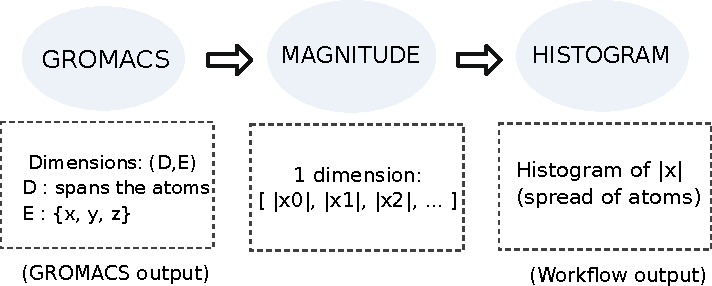
\includegraphics[width=\columnwidth]{fig/wflow_gromacs}
  \vspace{-0.25in}
  \caption{GROMACS Workflow}
  \label{fig:gromacs-workflow}
  \vspace{-0.15in}
\end{figure}


The three \sys workflows used in this evaluation performs
different kinds of runtime data analyses.
However, there are similarities.
First, each driving simulation 


\if 0
In this section we use
performance measurements on two of these workflows
to show (a) that a componentized method in
building workflows, which is inherent in the SuperGlue approach,
is valid from a performance point of view,
and (b) to show some of the scaling characteristics
of the components.
These results also serve to show that
SuperGlue workflows were successfully
deployed at various
scales.
% implicit here is that presenting
% performance measurements on the workflows
% shows more concretely that they actually *run*,
% which reinforces the statements in the
% previous section.

\if 0
The goals of the evaluation are to demonstrate the \ada{state goals
  clearly to set correct expectations, see if this is correct or needs
  to be expanded:} the feasibility of reusing
  SuperGlue components across workloads, and the ability of the
  SuperGlue components to maintain similar performance and scaling
levels as ``hand-tuned'' workflow compositions. 
\fi

The evaluation is performed on Titan, the Cray XK7 machine at Oak Ridge
National Laboratory. It consists of 18,688 nodes each with 1 16-core AMD
Opteron CPU and 32 GB of RAM. The interconnect is a Gemini network. There is an
attached Nvidia Kepler K20X GPU with an additional 6 GB of memory on every
node.

\subsection{Evaluation of Componentization}

\begin{table}[tbp]
  %\vspace{-0.15in}
  \centering
  \caption{LAMMPS SuperGlue vs. All-In-One Comparison}
  \label{tab:aio}
  \vspace{-0.07in}
  \begin{tabular}{|l|l|l|l|l|}
    \hline
    SIM output & AIO time (sec) & Superglue time (sec) & LMP only (sec) \\
    \hline
    20 MB & 115.26 & 116.51 & 115.03\\
    \hline
    80 MB & 148.70 & 149.80 & 146.97\\
    \hline
    320 MB & 154.65 & 157.65 & 153.69\\
    \hline
    1280 MB & 155.32 & 157.98 & 152.48\\
    \hline
    5120 MB & 167.39 & 168.79 & 165.22\\
    \hline
  \end{tabular}
  \vspace{-0.15in}
\end{table}

It is expected that assembling a workflow
using generic components involves the use
of finer-grain components
than when using ad-hoc analytical routines
specifically coded
for a workflow of interest.
One problem that might be anticipated
in more componentized workflows
is a decrease in overall performance caused by
(a) more stages that require the coordination
of readers and writers
and (b) more points of actual data transfer.

To investigate this potential problem,
we wrote a custom, all-in-one (AIO) component
that performs the same analytical procedure
as all the components involved in the LAMMPS workflow
(outside of the simulation itself, however).
We measured
the start-to-end completion times of the two workflows 
at different scales.

~\autoref{tab:aio} shows the start-to-end
completion times
at increasing scales, of
(a) LAMMPS with the AIO component
in the second column
(b) LAMMPS with the full SuperGlue workflow in the 3rd column
and (c) the LAMMPS simulation only with the output routines
removed from the code in the last column.
The measurements in the last column
are meant to give an idea of the portion
of the workflow completion time taken up by the simulation
computation only.

A weak scaling approach
is used, with approximately the same
per-process data size throughout the scaling.
The time is measured from the start of the simulation
to the point when the last histogram of
the last timestep is written.
For each SuperGlue workflow run, the corresponding
AIO workflow run allocates the same
number of processes to the AIO component
as the SuperGlue workflow allocates to the Select component.
In the SuperGlue workflow, additional processes
are allocated to the other two components
(Magnitude and Histogram).

The results show only a small increase in
workflow completion time for the SuperGlue
workflows (with a maximum increase of $1.9 \%$).
As mentioned previously, the componentized
approach involves more data exchange points
in the workflow, thus leading to
overhead from increased $MxN$ coordination and data exchange.
However, FlexPath allows
for asynchronous data transfer.
More specifically, when a writer writes to
a ``stream,'' it places
the data in an internal buffer
until the readers are ready to request it,
at which point a separate thread in the writer
handles the actual transfer.
This overlap
of computation and I/O
amortizes the aforementioned overhead.

Also, in the SuperGlue workflow,
the componentization of the analysis
allows for a higher level of parallelism in the overall
analysis. As an example, in the AIO component,
the Select stage of one timestep
only begins once the Magnitude
stage of the previous timestep
completes, since they exist in the same processes.
In the SuperGlue workflow, these
computational stages can run simultaneously.

Granted, more resources are allocated to the
SuperGlue workflow runs to allow the additional
components to execute.
Also, much of the start-to-end time is spent on
the simulation's computation.
However, the measurements in the last column
of \autoref{tab:aio}
only give an idea of the proportion of 
overall time occupied by the simulation only,
since when workflows are running, there is much
overlap in the computation and I/O between the
simulation and other components.
All in all, this is
an illustrative comparison that shows the validity,
from a performance angle,
of the componentized approach
to building workflows.

\subsection{Scaling}

\begin{table*}[tbp]
  \centering
  \caption{GTCP Evaluation Configuration Settings}
  \label{tab:eval-strong-gtcp}
  \vspace{-0.05in}
  \begin{tabular}{|l|l|l|l|l|l|}
    \hline
    Component Test & GTCP Procs & Select Procs & Dim-Reduce 1 & Dim-Reduce 2 & Histogram Procs \\
    \hline
    Select & 64 & $x$ & 4 & 4 & 4\\
    \hline
    Dim-Reduce 1 & 128 & 32 & $x$ & 16 & 16\\
    \hline
    Dim-Reduce 2 & 128 & 32 & 16 & $x$ & 16\\
    \hline
    %Histogram & 128 & 34 & 24 & 24 & $x$\\
    %\hline
  \end{tabular}
  \vspace{-0.07in}
\end{table*}

\begin{figure}
  \centering
  %\vspace{-0.17in}
  \input{data/gtcp-sel1-strong}
  %\vspace{-0.17in}
  \input{data/gtcp-dimr-strong}
  %\vspace{-0.06in}
  \caption{SuperGlue strong scaling in the GTCP workflow. Whole timestep
    completion time (secs) for Select and both instances of Dim-Reduce used in
    the workflow are plotted against process size}
  \label{fig:gtcp-strong}
  \vspace{-0.25in}
\end{figure}

We carried out a number of experiments
to determine some of the strong and weak scaling
characteristics of the components.

Strong scaling measurements are useful for
determining appropriate process sizes
for the components, based on the size of the
data set they operate on.
For these strong scaling measurements,
we varied the process size of a single component at
a time while fixing that of the
other components involved in the workflow,
all the while using a fixed output size from
the driving simulation.
We timed the completion of a whole timestep
taken arbitrarily in the middle of the workflow
of one component of interest at a time,
taking an average over all processes
involved in that component's timestep.

In~\autoref{fig:gtcp-strong} we show some results 
from the GTCP workflow.
The corresponding configurations (process sizes for all components)
that were used to obtain these results are listed
in~\autoref{tab:eval-strong-gtcp}.
These strong scaling results show a general trend
seen in the strong scaling experiments for SuperGlue
components: a linear domain of scalability followed
by a turning point and eventual flattening
of the curve. This shows
that given
a particular workload, users can select SuperGlue process sizes
that match their resources and performance requirements.

Similar measurements exist for the LAMMPS and GROMACS workflows.
These are available in the repository~\cite{champsaur:superglue-repo}.

The third column of~\autoref{tab:aio} already
shows promising
weak scaling characteristics of SuperGlue
in the LAMMPS workflow. That is, there is little
difference in the end-to-end
completion time of the workflow
for simulation output sizes varying
from 80 MB to 5120 MB (a factor of 64
increase in simulation output size).
For the 5120 MB run, the configuration used
was 1024 LAMMPS processes, 256 Select processes,
256 Magnitude processes, and 64 Histogram processes.

Per-component, per-timestep results
showing good weak scaling characteristics of
SuperGlue
also exist for the GTCP workflow and are also
available in~\cite{champsaur:superglue-repo}.
Space limitations prevent us
from showing them here.

\if 0
\subsection{Strong Scaling Experiments}


\begin{figure}
  \centering
  \vspace{-0.25in}
  \input{data/lmp-sel-strong}
  \vspace{-0.15in}
  \input{data/lmp-mag-strong}
  \vspace{-0.17in}
  \input{data/lmp-hist-strong}
  %  }
  %
  \vspace{-0.05in}
  \caption{SuperGlue strong scaling in the LAMMPS workflow.
    Completion time (secs) of a full timestep and of the data transfer
    portion of the same timestep are plotted against process size.}
  \label{fig:lammps-strong}
  \vspace{-0.18in}
\end{figure}

\begin{figure}
  \centering
  \vspace{-0.17in}
  \input{data/gtcp-sel1-strong}
  \vspace{-0.17in}
  \input{data/gtcp-dimr-strong}
  \vspace{-0.06in}
  \caption{SuperGlue strong scaling in the GTCP workflow. Whole timestep
    completion time (secs) for Select and both instances of Dim-Reduce used in
    the workflow are plotted against process size}
  \label{fig:gtcp-strong}
  \vspace{-0.25in}
\end{figure}

\ada{add axis labels and units to plots. }
  

\begin{table*}[tbp]
%\vspace{-0.15in}
\centering
\caption{LAMMPS Evaluation Configuration Settings}
\label{tab:eval-strong-lammps}
\vspace{-0.15in}
\begin{tabular}{|l|l|l|l|l|}
\hline
Component Test & LAMMPS Procs & Select Procs & Magnitude Procs & Histogram Procs \\
\hline
Select & 256 & $x$ & 16 & 8\\
\hline
Magnitude & 256 & 60 & $x$ & 8\\
\hline
Histogram & 256 & 32 & 16 & $x$\\
\hline
\end{tabular}
%\vspace{-0.15in}
\end{table*}

%LAMMPS setups:
%Select is 256:x:16:8
%Magnitude is 256:60:x:8
%Histogram is 256:32:16:x

\begin{table*}[tbp]
\centering
\caption{GTCP Evaluation Configuration Settings}
\label{tab:eval-strong-gtcp}
\vspace{-0.15in}
\begin{tabular}{|l|l|l|l|l|l|}
\hline
Component Test & GTCP Procs & Select Procs & Dim-Reduce 1 & Dim-Reduce 2 & Histogram Procs \\
\hline
Select & 64 & $x$ & 4 & 4 & 4\\
\hline
Dim-Reduce 1 & 128 & 32 & $x$ & 16 & 16\\
\hline
Dim-Reduce 2 & 128 & 32 & 16 & $x$ & 16\\
\hline
%Histogram & 128 & 34 & 24 & 24 & $x$\\
%\hline
\end{tabular}
\vspace{-0.07in}
\end{table*}

%GTCP setups:
%Select is 64:x:4:4:4
%Dim-Reduce1 is 128:32:x:16:16
%Dim-Reduce2 is 128:32:16:x:16
%Histogram is 128:34:24:24:x

To understand the strong scaling behavior exhibited by the components in
different scenarios, we carried out strong scaling measurements of the
components in both the LAMMPS and GTCP workflows.
To do this, we varied the process size of a single component at
a time while fixing that of the other components involved in the workflow,
and using a fixed output size from the driving simulation.  We
determined reasonable process sizes for the fixed-size components using
preliminary testing. 

The results are illustrated in~\autoref{fig:lammps-strong} and~\autoref{fig:gtcp-strong}.
Each point shows
the completion time for a single time step arbitrarily chosen in the middle of
the execution of the workflow. Depicted below the strong scaling curves
in~\autoref{fig:lammps-strong}
are the data transfer times. That is, these points
show the portion of the timestep
completion time spent by the components waiting to receive requested data.
The workflow configurations (process counts) used to obtain these measurements are shown
in~\autoref{tab:eval-strong-lammps} and~\autoref{tab:eval-strong-gtcp}.
The global output of the simulation in the LAMMPS workflow
is \SI{1.28}{\giga\byte}. In the GTCP workflow, the Select
measurements are taken using a \SI{900}{\mega\byte} output
from the simulation, and those of Dim-Reduce using a
\SI{3.8}{\giga\byte} output.
The scale used for these results is small compared to the
scale at which these simulations can be run due to
the limited time and resources available 
for the numerous complete workflows executions required
to obtain meaningful strong scaling results.

These results provide valuable information about the components.
First, they show that the components exhibit regular strong
scaling behavior. That is, 
a linear domain of scalability is followed by a turning point and an
eventual flattening out of the performance, where the benefit
of adding more processes dwindles.
That there exists a linear domain means that given
a particular workload, users can select SuperGlue process sizes
that match their resources and performance requirements.
The flat domain is long and does not show any drastic reversal
of performance. Without knowing the full strong
scaling characteristics of the SuperGlue components used in a particular workflow,
a user can safely guess a process size to use for a particular component,
using the strong scaling results from the same component with a similar
workload size, without incurring unreasonable overhead.

The turning point of scalability of a component
is not necessarily determined by
its per-process workload size.
In~\autoref{fig:lammps-strong}, the turning point of Select
occurs at a per-process workload of around \SI{32}{\mega\byte}.
Here, the global data size sent to Select
is \SI{1.28}{\giga\byte}.
In a separate set of measurements using the GTCP workflow,
the turning point of Select occurs at a per-process workload
of \SI{113}{\mega\byte}, where the global dataset size
was \SI{3.8}{\giga\byte}. Therefore, global workload size
is a factor in determining the turning point of scalability
of the SuperGlue components.

While there is communication overhead in the computation itself,~\autoref{fig:lammps-strong} shows the majority of the communication
overhead, i.e., the time spent on data transfer between components,
is small compared to the total per-timestep execution time of
the SuperGlue components. This supports the idea
of assembling workflows using numerous, simple,
generic components.

\subsection{Weak Scaling Experiments}

Additional experiments are performed for the GTCP workflow to determine the
weak scaling performance for the components. The configurations for these experiments
are presented in~\autoref{tab:eval-weak-gtcp-1}. The performance results are
presented in~\autoref{tab:eval-weak-gtcp-2}. To read the tables, match the
rows. For example, the first row in~\autoref{tab:eval-weak-gtcp-1} corresponds
to the performance results in row 1 in~\autoref{tab:eval-weak-gtcp-2}.
These runs use SuperGlue process sizes for which the per-process
workloads reside near the turning points in the
strong scaling results presented above.

Overall, the components and the overall workflow
exhibit very promising weak scaling behavior.
While there are slightly different per-process
data sizes in each row of the table for both
per-simulation process and per-SuperGlue process,
there is little variation in the timestep completion
times of the SuperGlue components and in the end-to-end
completion times of the entire workflow for different
workload sizes.

{\em Select} gets the full brunt of the total data size. Dividing the process
count into the total data size shows that on average, it is roughly the same
for weak scaling. The other components exhibit similar performance consistency.
Also note that these are not exactly identical ratios or counts.  The data size
per GTCP process is maintained as it is scaled. The amount of data each
SuperGlue component process varies a bit. Also note that there is not a fixed
n-1 ratio required for any of the components. Instead, an m-n mapping works
correctly.

%Process count ratios
%GTCP	GTCP		GTCP
%vs	vs		vs
%Select	Dim-Reduce	Histogram
%6.4	10.67		32
%5.25	8.4		41
%8.67	11.14		34
%9.36	12.31		46.8

\begin{table*}[tbp]
%\vspace{-0.15in}
\centering
\caption{GTCP Weak Scaling Evaluation Configuration Settings}
\label{tab:eval-weak-gtcp-1}
\vspace{-0.15in}
\begin{tabular}{|l|l|l|l|l|l|l|l|}
\hline
Configuration & GTCP Procs & Select Procs & Dim-Reduce 1 & Dim-Reduce 2 & Histogram Procs & Total Data Size & End-to-End Time\\
\hline
C1 & 64 & 10 & 6 & 6 & 2 & 918,303,680 & 92.724\\
\hline
C2 & 84 & 16 & 10 & 10 & 2 & 1,434,599,936 & 115.232\\
\hline
C3 & 156 & 18 & 14 & 14 & 4 & 2,065,583,520 & 97.266\\
\hline
C4 & 234 & 25 & 19 & 19 & 5 & 2,811,256,000 & 96.359\\
\hline
\end{tabular}
\vspace{-0.15in}
\end{table*}

\begin{table}[tbp]
%\vspace{-0.10in}
\centering
\caption{GTCP Weak Scaling Component Performance}
\label{tab:eval-weak-gtcp-2}
\vspace{-0.15in}
\begin{tabular}{|p{0.1 in}|p{0.67 in}|p{0.65 in}|p{0.65 in}|p{0.65 in}|}
\hline
 & Select Average Time & Dim-Reduce 1 Average Time & Dim-Reduce 2 Average Time & Histogram Average Time\\
\hline
C1 & 1.55 & 1.58 & 1.34 & 0.6\\
\hline
C2 & 2.34 & 1.58 & 1.72 & 0.78\\
\hline
C3 & 2.31 & 1.73 & 1.54 & 0.713\\
\hline
C4 & 2.19 & 1.76 & 1.68 & 0.89\\
\hline
\end{tabular}
\vspace{-0.25in}
\end{table}

\fi
\fi

%\section{Discussion}
\label{s:discuss}

%\section{Related work}
\label{s:relwk}

%\section{Conclusions and Future Work}
\label{s:conclusion}

This paper presents SuperGlue, a demonstration of making generic, reusable
components for scientific simulations. By decomposing the operations into small
chunks, we achieve components that can be reused, without modification, for
a variety of different workflows. In this work, we investigate using a
stream-based structure with generic components to achieve easier to build and
use workflows.  Stream-based, generic workflow components should be designed 
to allow the greatest variety in their arrangement and for a maximum
number of downstream subscribers. Designing components with the ability to
handle data having any number of dimensions provides a very useful way to link
them together. Maintaining a high level of semantics upstream, for example by
labeling dimensions and certain quantities inside of these dimensions, gives a
good understanding of the data to downstream components. There is a need for
components that organize the data in a format that downstream components can
understand.

Through the demonstration of generating a velocity histogram for LAMMPS,
a pressure histogram for GTCP,
and a distribution of the spread of the atoms for a GROMACS
experiment,
we demonstrate reusing the same components
over different data formats and application types.

While this work leverages ADIOS and the FlexPath transport, this is not the
only approach for addressing reusable components. Other, similar approaches can
also work well. However, in this case, the data annotation provided by this
connection infrastructure helps enable reusable components by offering
necessary metadata to perform general operations.

Future work involves
expanding the generic components library 
to include a variety of analytical operations.
In particular, the SuperGlue components presented
in this paper
result in an output dataset having either the same
size or a smaller size as the input.
Analytical procedures that lead
to an increase in data size, such as
all-pairs calculations, are common and
can be implemented using the SuperGlue approach.

Also common are operations that require the in-memory
buffering of a dataset throughout a series
of timesteps. An example of this is the
calculation of root-mean-square
deviations of atomic positions from a fixed,
starting set of positions.

Two current limitations of SuperGlue are
that 
all components are launched at once and
workflows cannot branch.

To turn SuperGlue into a true Workflow Management
System, we hope to leverage
ADIOS' ability to have several ``write groups''
so as to allow for the development
of a {\em Fork} component
that would permit
the creation of workflows
described by directed acyclic graphs.
And, to manage the execution of workflows
over longer periods of time,
we plan on investigating
the incorporation of SuperGlue into
higher-level workflow management systems
such as Kepler and DAGMan.

The components we have developed in this research cover only a small portion of
the procedures that computational scientists need for their
workflows. Eventually, we wish to allow for the development of a large
collection of generic workflow components. We can take steps in this direction
by building on our existing components. For example, {\em Magnitude} performs a
relatively simple operation on multi-dimensional data, where one dimension
spans a number of quantities involved in each instance of the operation. This
model can fit any number of operations involving a repeating, fixed number of
quantities, and it can even be made to work with a formula specified by the
user at runtime. This opens the door to a large family of generic components.

\if 0
Finally, while we have kept performance in mind in the development of these
components, performance optimization is not yet the focus of this research. In
the design of any generic tool however, the question of performance inevitably
arises. Indeed, designing tools that are not meant to operate on a specific
format of input data can easily impact performance. For example, {\em
Dim-Reduce} performs the same amount of computation whether it re-arranges data
or not. In the long run, optimizing these components will involve detecting
such situations where they can avoid performing unnecessary iterations and data
manipulation.
\fi

\section*{Acknowledgments}

%
\includegraphics[scale=0.07]{logos/doe_logo}
%
\includegraphics[scale=0.30]{logos/snl_logo}
%
\includegraphics[scale=0.35]{logos/nnsa_logo}
Sandia National Laboratories is a multi-program laboratory managed and operated
by Sandia Corporation, a wholly owned subsidiary of Lockheed Martin
Corporation, for the U.S. Department of Energy's National Nuclear Security
Administration under contract DE-AC04-94AL85000.

This work was supported by Advanced Scientific Computing Research, Office of
Science, U.S. Department of Energy, under Contract DE-AC02-06CH11357, program
manager Lucy Nowell.


%\balance
\bibliographystyle{IEEEtran}
\footnotesize
\bibliography{gcomps,p,fakeroot,sslab,manycore,conf}
\end{document}
